\documentclass[12pt]{article}
\usepackage[a4paper,left=2.5cm,right=2.5cm,top=\dimexpr15mm+1.5\baselineskip,bottom=2cm]{geometry}
\usepackage[T1]{fontenc}
\usepackage[utf8]{inputenc}
\usepackage{geometry}
\usepackage{fancyhdr}
\usepackage{graphicx}
\usepackage{lmodern}
\usepackage[portuguese]{babel}

\renewcommand{\headrulewidth}{.4mm} % header line width

\pagestyle{fancy}
\fancyhf{}
\fancyhfoffset[L]{1cm} % left extra length
\fancyhfoffset[R]{1cm} % right extra length
\rhead{\today}
\lhead{\bfseries SIBD}
\rfoot{}

\begin{document}
\noindent Etapa 1\\
Grupo 28\\
\\
João Ricardo Silva Matos nº 56292 Turma 02\\
João Pedro Ramos Vedor nº 56311 Turma 02\\
João Gonçalo Jorge dos Santos nº 57103 Turma 01\\
Daniel Caetano Luís nº 56362 Turma 01\\

\begin{figure}[h]
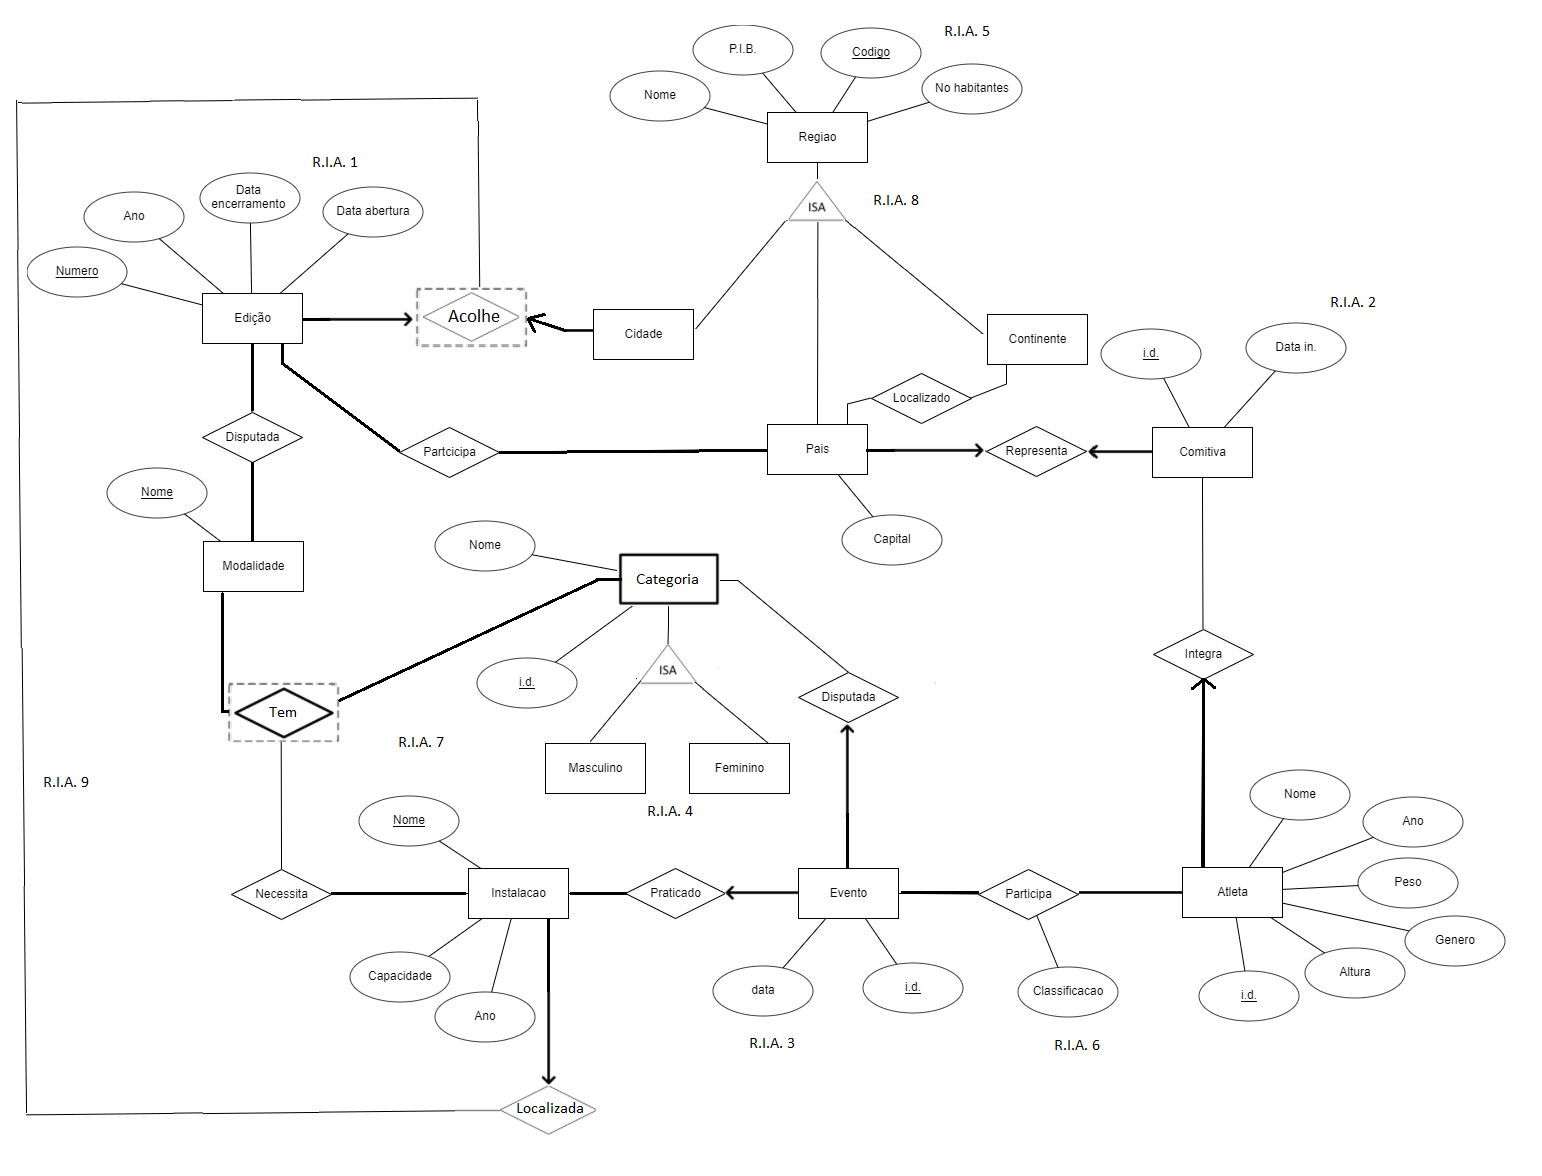
\includegraphics[scale=0.45, angle =90]{image.png}
\end{figure}



\newpage

\noindent Etapa 1\\
Grupo 28\\
\\
João Ricardo Silva Matos nº 56292 Turma 02\\
João Pedro Ramos Vedor nº 56311 Turma 02\\
João Gonçalo Jorge dos Santos nº 57103 Turma 01\\
Daniel Caetano Luís nº 56362 Turma 01\\
\\
Restrições de Integridade adicionais:
\begin{itemize}
\item[1] A data de encerramento deve ser posterior á data de abertura
\item[2] A data de inscrição deve ser anterior á data de abertura da edição
\item[3] A data do evento deve ser posterior á data de abertura da edição e anterior á data de encerramento da mesma
\item[4] Masculino and Feminino cover Categoria
\item[5] O código deve ser composto por 3 letras maiúsculas
\item[6] A primeira posição na classificação atribui uma medalha de ouro, a segunda uma de prata, e  terceira uma de bronze
\item[7] Os eventos de uma categoria são praticados numa instalação, sendo que esta tem o pré-requisito de poder receber eventos dessa categoria
\item[8] Cidade and País and Continente cover Região
\item[9] A instalação fica localizada na cidade que acolhe a edição
\end{itemize}
\end{document}